\documentclass[12pt]{article}

%% preamble: Keep it clean; only include those you need
\usepackage{amsmath}
\usepackage[margin = 1in]{geometry}
\usepackage{graphicx}
\usepackage{booktabs}
\usepackage{natbib}

% for space filling
\usepackage{lipsum}
% highlighting hyper links
\usepackage[colorlinks=true, citecolor=blue]{hyperref}


%% meta data

\title{Examining Various Statistical Methods in Predicting Loan Default}
\author{Chris Truedson\\
  Department of Statistics\\
  University of Connecticut
}

\begin{document}
\maketitle

\begin{abstract}
TBD  
\end{abstract}


\section{Introduction}
\label{sec:intro}

Approximately 22.7 million Americans have personal loans, 45 million have student loans, and 51.5 million households have mortgages with the vast majority of all these loans coming from banks and similar financial institutions. As such, it is crucial that these businesses are able to efficiently, accurately, and with the greatest level of optimization determine who it is safe to loan money to and who is likely to default. This is a practical business problem that is continuously being tinkered with to find new and better approaches. Many studies have took on the issue of using machine learning to predict whether a customer will default on a loan or not using various different methods like decision trees and random forests \citet{madaan2021loan}, KNN approaches \citet{lai2020loan}, and deep neural nets \citet{bayraci2019deep} to name a few.

% roadmap
The rest of the paper is organized as follows.
The data will be presented in Section~\ref{sec:data}.
The methods are described in Section~\ref{sec:meth}.
The results are reported in Section~\ref{sec:resu}.
A discussion concludes in Section~\ref{sec:disc}.


\section{Data}
\label{sec:data}

The data I'll be using primarily will come from the \href{https://www.kaggle.com/datasets/nikhil1e9/loan-default}{Loan Default Prediction Dataset} on Kaggle. Itself is a dataset from a Coursera competition \href{https://www.coursera.org/projects/data-science-coding-challenge-loan-default-prediction}{Loan Default Predicition Challenge} featuring 255,347 observations and 18 variables with various demographic and financial data including but not limited to the borrowers age, their income, their education, their credit score, the loan amount, the type of loan, and various other metrics which provide a full picture of the loan, the borrower, and the borrower's financial situation.

\section{Methods}
\label{sec:meth}

Use this section to present the methodologies that will generate results by
analyzing the data. Suppose that the radius of a circle is $r$. Then its area is
\begin{equation}
  \label{eq:area}
  \pi r^2.
\end{equation}

Equation~\eqref{eq:area} is interesting. \lipsum[1-4]

Sometimes I don't want an equation to be numbered such as this one:
\[
  f(x) = \frac{1}{\sqrt{2\pi}} \exp\left( - \frac{x^2}{2} \right),
\]
which is the density of a standard normal variable.



\section{Results}
\label{sec:resu}

Table~\ref{tab:rv} summarizes some example draws from some distributions.
\lipsum[1-4]

\begin{table}[tbp]
  \caption{This is my first table.}
  \label{tab:rv}
\centering
\begin{tabular}{rrr}
  \toprule
normal & poisson & gamma \\ 
  \midrule
-0.110 & 4 & 2.401 \\ 
  0.116 & 4 & 3.529 \\ 
  -0.828 & 9 & 2.112 \\ 
  -0.066 & 6 & 11.104 \\ 
  0.219 & 3 & 4.815 \\ 
  0.303 & 5 & 2.188 \\ 
  0.544 & 0 & 8.050 \\ 
  -2.617 & 8 & 3.646 \\ 
  0.747 & 1 & 5.178 \\ 
  -1.103 & 4 & 3.043 \\ 
   \bottomrule
\end{tabular}
\end{table}

Figure~\ref{fig:cars} shows the distance against the speed from this dataset.


\begin{figure}[tbp]
  \centering
  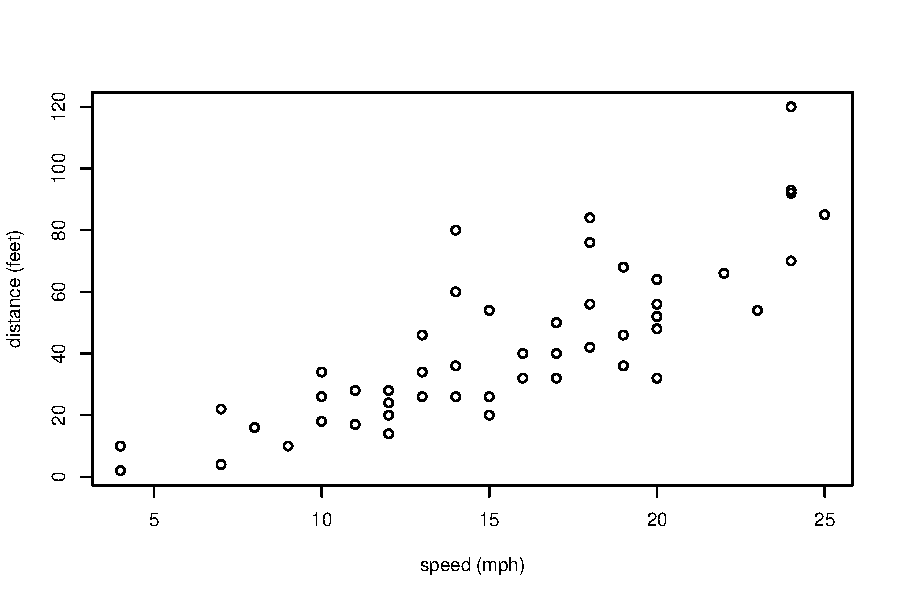
\includegraphics[width=\textwidth]{cars.pdf}
  \caption{This is my first figure.}
  \label{fig:cars}
\end{figure}

\section{Discussion}
\label{sec:disc}

The most challenging parts of the proposed work will be fitting and tuning each of the models. While straightforward in building them each model will require tuning using a variety of techniques. More difficult still will be testing more models than just those that have been proposed with perhaps even more specialized and advanced machine learning models like deep neural networks and even extreme gradient boosting as discussed in \citet{lai2020loan}. 
\par The limitations of my work are twofold. With regards to my first aim of finding the most important variables, the dataset I'm working with contains 18 of probably the most common types of variables used in this setting however, other critical variables may be missing making my work in finding the most significant variables and seeing if they change with the type of loan bounded. In regards to my second aim of finding the "best" model, there's many limitations such as I won't be testing ALL possible models, instead I'll only be testing the most common and relatively simple with the possibility for some less employed more advanced models to be tested as well. Additionally, the dataset while "large" at approximately 250,000 observations businesses could be working with datasets magnitude of this size which if the models prove to all be very effective with very minor accuracy changes between them could see a shift in a much larger dataset of the "best" model.  
\par Overall, I expect this project to go relatively smoothly as the project while it has complex components depending on the models employed and the level of tuning at the most base level is relatively straightforward. If things do go wrong for whatever reason there were multiple other datasets I found with similar variables and looking at default prediction which could be used to replace or even compliment potentially my current dataset.

\bibliography{refs}
\bibliographystyle{mcap}

\end{document}